\section{Discussion}

\subsection{Why ML-DSA Is the Practical Default}

ML-DSA fits the firmware-signing use case because it offers a manageable compromise between cryptographic conservatism and deployment cost. Its signatures are much larger than ECDSA, but they remain in a range that can be tolerated by many update formats and manifests. In contrast, SLH-DSA signatures quickly become dominant on small images. If a platform must choose one PQ signature family for broad deployment today, ML-DSA is therefore the most pragmatic default.

\subsection{Why SLH-DSA Still Matters}

It would be a mistake to dismiss SLH-DSA merely because its signatures are large. NIST standardized it specifically as a backup that relies on a different mathematical basis than ML-DSA \cite{nist_pqc_release}. In high-assurance environments, that diversity is valuable. A vendor may decide to keep SLH-DSA support for recovery tooling, high-value product lines, or contingency planning even if ML-DSA is the main production choice.

\subsection{When Dual Signatures Are Justified}

Dual signatures are justified when compatibility requirements are real and temporary. They are especially useful when the installed base contains immutable verifiers that understand only classical signatures while newer devices can already verify PQ signatures. However, dual signatures should be paired with either a both-required rule or an authenticated version-gated rule. Otherwise the transition accumulates cryptographic baggage without actually removing classical exposure.

\begin{figure}[H]
\centering
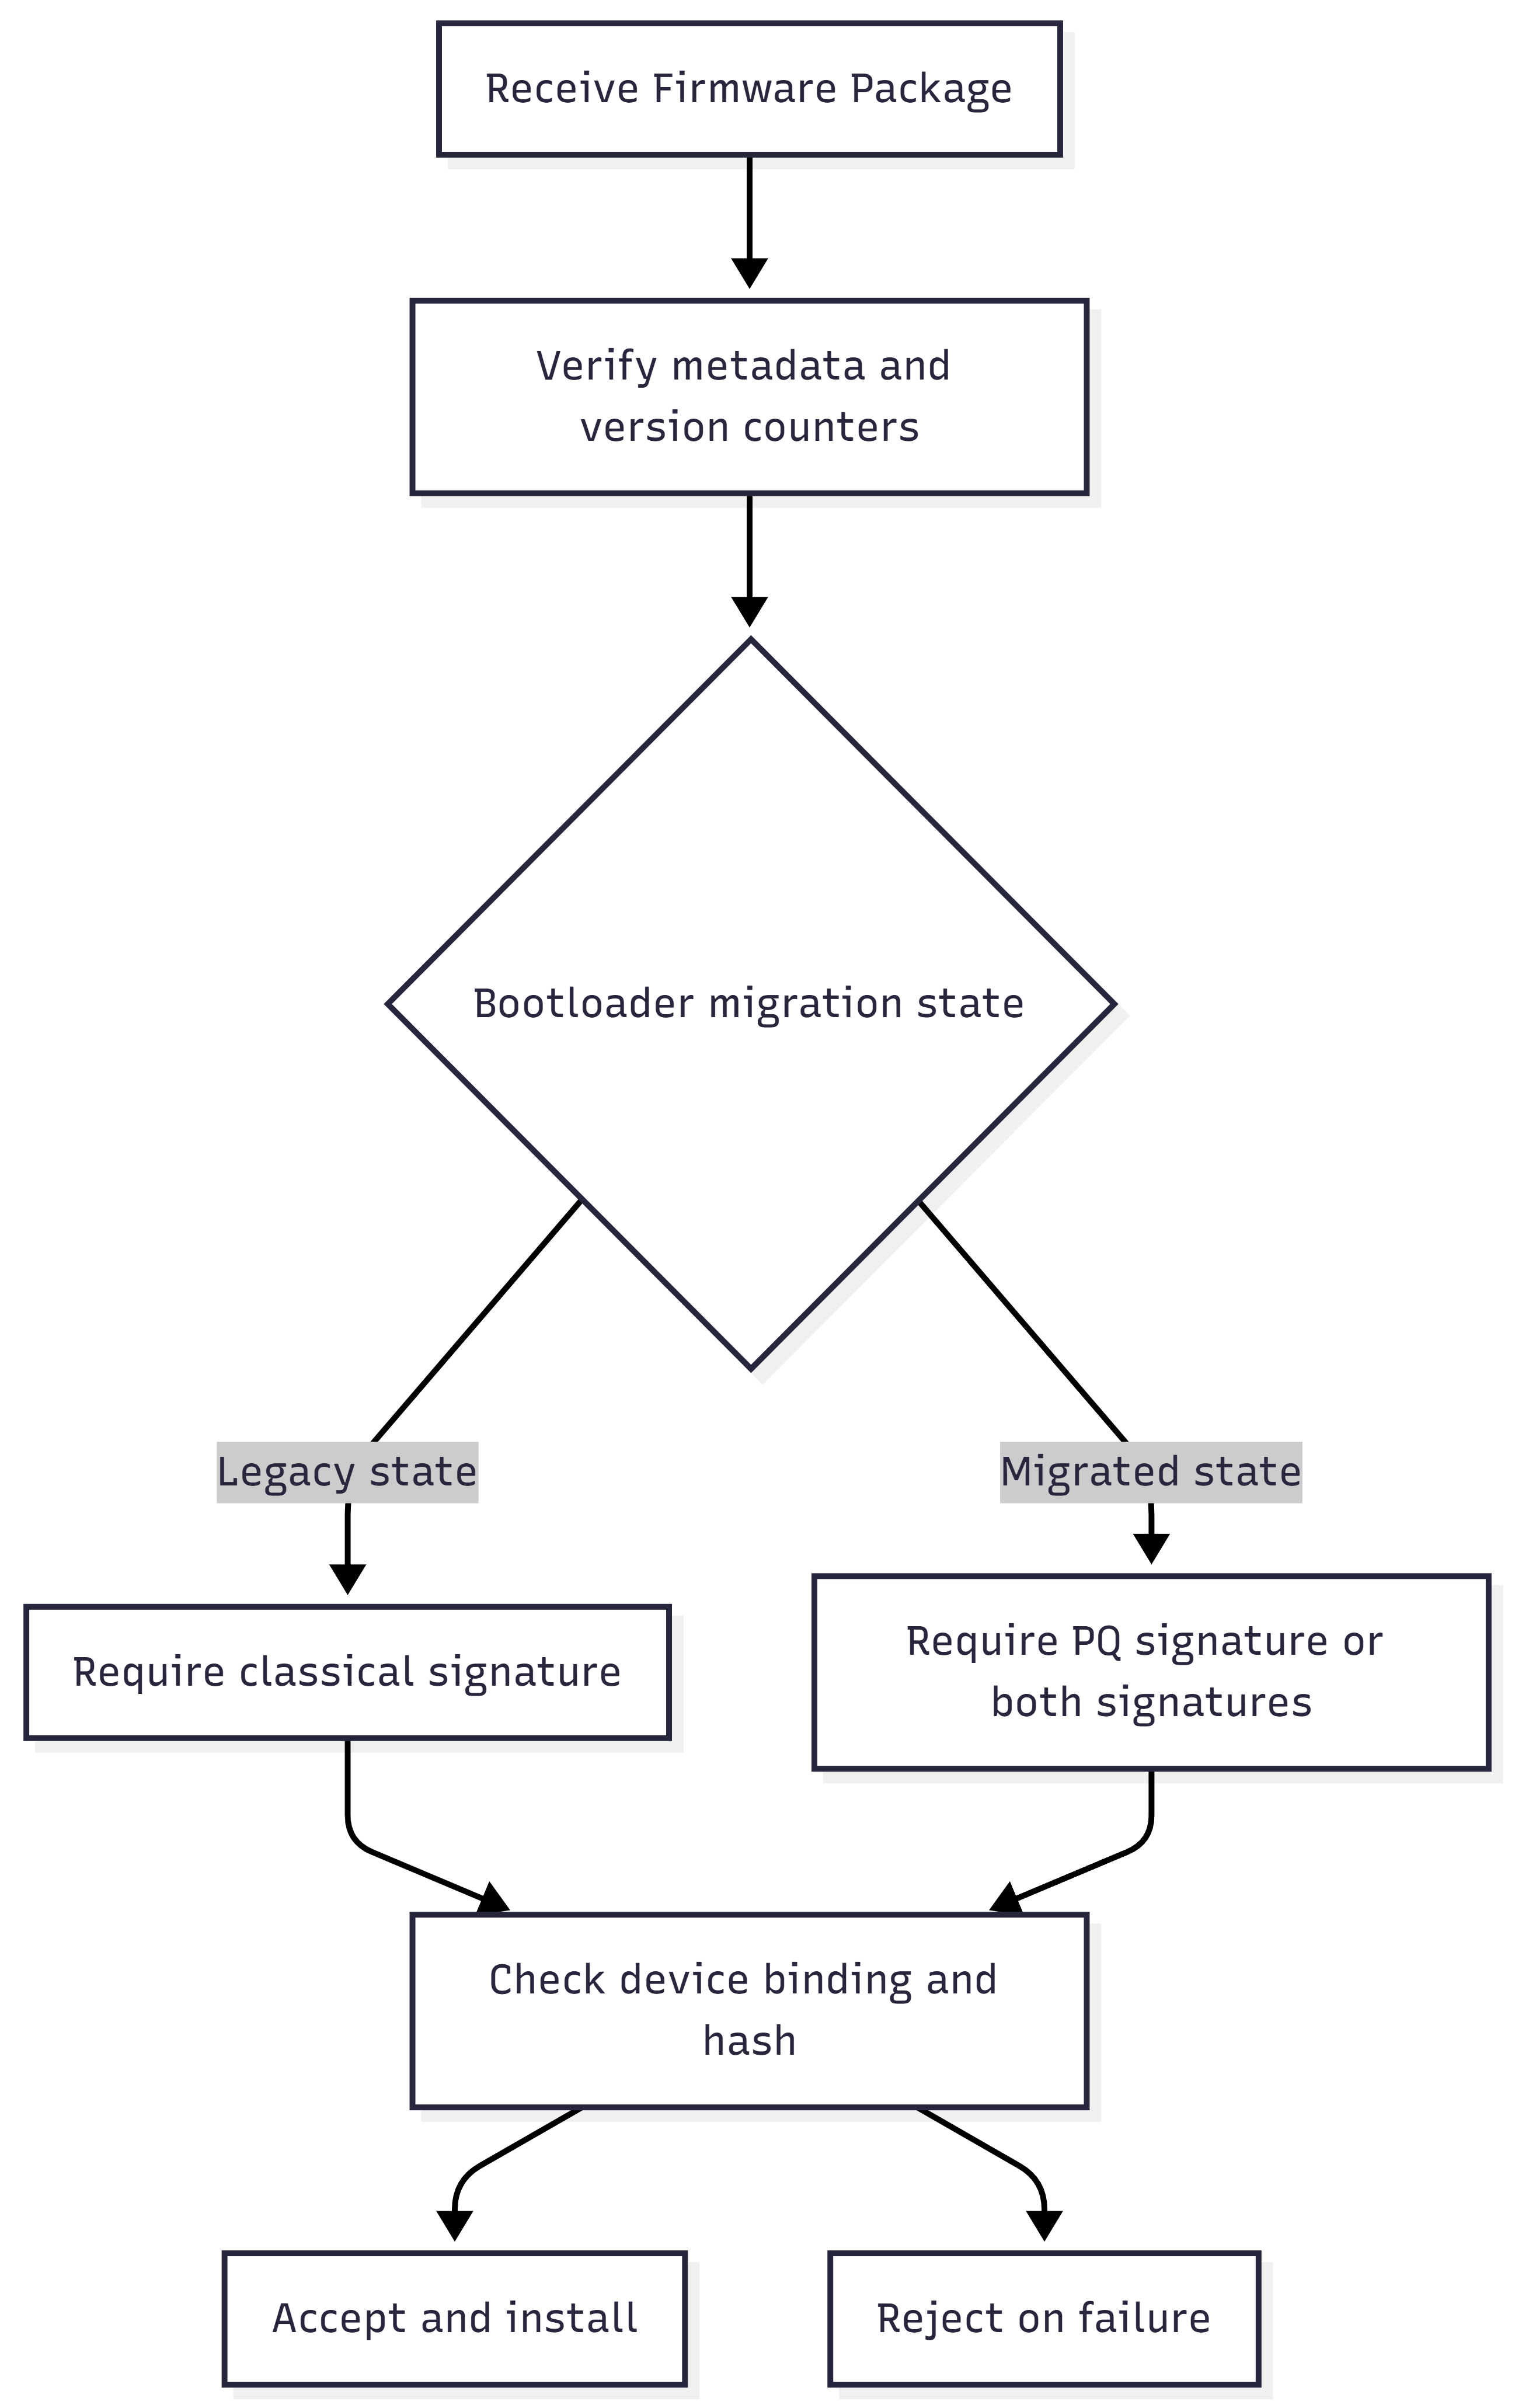
\includegraphics[width=0.9\columnwidth]{../images/policy.png}
\caption{Migration-policy flow for legacy and post-migration verification states.}
\label{fig:migration}
\end{figure}

\subsection{Limitations}

This study has two main limitations. First, it does not present cycle-accurate embedded benchmarks for ML-DSA or SLH-DSA on a specific microcontroller. Instead, it focuses on deployment-visible metrics that can be derived directly from the finalized standards and from policy logic. Second, the prototype treats signature validity abstractly; it models the presence of valid signatures rather than invoking a concrete PQC implementation.

These limitations are acceptable for the scope of this paper because the central claim is architectural: secure migration depends on authenticated metadata and downgrade-resistant policy, not only on choosing a larger or smaller signature. Future work can extend the prototype with real verifier benchmarks on an embedded platform and with certificate-chain modeling for production firmware ecosystems.
